\section{Существующие решения}

\subsection{Обзор методов сетевого мониторинга ядра Linux}

В данном разделе рассмотрены основные подсистемы и средства сетевого мониторинга ядра Linux, которые используются в настоящее время. Все они различаются по своим особенностям и применяемым технологиям. Данные методы имеют ряд своих преимуществ и недостатков при решение определенной задачи по мониторингу сетевой подсистемы, в частности контролированию пути и обработки сетевого пакета.

\subsubsection{Утилиты для сетевого мониторинга}
Для современных Linux существует множество утилит для конфигурации и устранения неполадок сетевой подсистемы ядра. 
В основном это инструменты командой строки.  
Наиболее распространенные и часто используемые из них iproute2, ethtool, ping, traceroute, nslookup, netcat, iptables, tcpdump \cite{tcpip_craig}, с помощью которых можно узнать конфигурацию сетевых пакетов, проверить наличие соединения и работоспособность Domain Name System (DNS), просмотреть таблицу маршрутизации, изучить содержание сетевых пакетов и многое другое, что может помочь определить сбои в сетевой подсистеме.

Путем использования данных утилит с одной стороны обеспечивает безопасность и производительность, но с другой --- такое множество средств заточено под определенную задачи и их функциональность ограничена программным интерфейсом ядра Linux.
Многие инструменты имеют документацию, благодаря которой можно разобраться для чего необходимо и как использовать утилиту. 
Все же решая какую-либо сложную задачу, а многие задачи мониторинга сетевой подсистемы и есть такие, поэтому необходимо использовать комбинацию данных утилит, если такие утилиты имеются.

\subsubsection{Модификация кода ядра Linux}
Открытость ОС Linux позволяет реализовать средства получения информации о событиях, происходящих в сетевой подсистеме ядра, путем модификации исходного кода ядра, что дает возможность находить сбои.

Модификация ядра Linux --- изменение или добавление кода, которое не несет изменение структур ядра Linux. Модификация с целью сетевого мониторинга изменение кода сетевой подсистемы ядра Linux, путем добавление функционала вывода информации в системный журнал.~\cite{linux_network_implementation}

Для отслеживания пути пакетов необходимо разместить код, перехватывающий события <<ловушки>> и выводимые информацию либо в системный журнал, либо в пользовательское приложение. 
На рисунке~\ref{img:ex_mod} показан пример структуры добавление кода в ядро Linux для отслеживания пути пакета, где модуль регистрации событий --- динамически загружаемый модуль ядра Linux.
Каждая ловушка сигнализирует о конкретном событии с конкретным пакетом, поэтому в обработчик перехваченных событий передается идентификатор пакета, место возникновения события, код события и дополнительная параметры. В качестве идентификатора пакета используется структура sk\_buff, в которой содержатся пакет. Ловушки размещаются в начале и в конце сетевых функции фильтрации обрабатываемых пакетов в случае удовлетворению фильтра вывод необходимой информации. Благодаря чему можно определить как изменился пакет при возникновении ошибки и к чему это привело.~\cite{ip_monitoring}

\begin{figure}[h!]
	\centering
	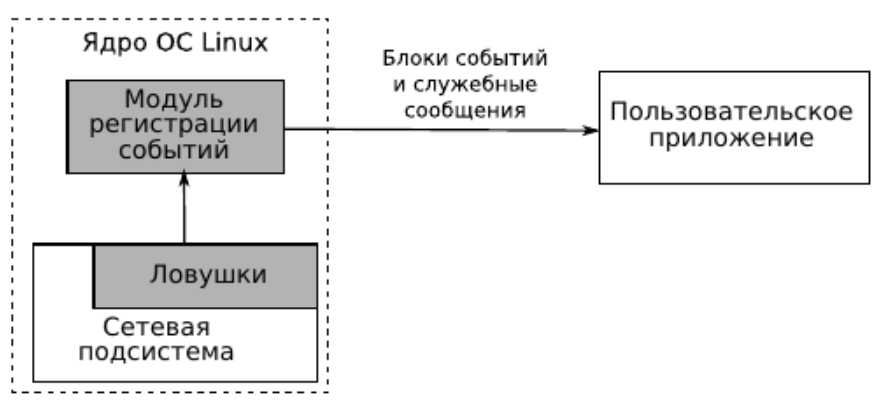
\includegraphics[height=0.3\textheight]{img/ex_mod} % height
	\caption{Структурная схема системы слежения пути пакета}
	\label{img:ex_mod}
\end{figure}

Модификации ядра имеют доступ ко всему функционалу, включая системные вызовы.
При неверном изменении кода ядра возникают критические ошибки, которые могут привести к нарушению работоспособности системы, вследствие чего нельзя достичь необходимого уровня безопасности.
Кроме того для добавления кода в ядро необходимо обладать профессиональными навыками работы с языком С и компилятором с инструментами конфигурации ядра.
Модификация и пересборка ядра делают невозможный запуск на реальной системе, что делает процесс длительным и осложненным при достижении низких расходных ресурсов при фильтрации пакета в каждой функции ядра.
Но с другой стороны модификация кода дает возможность решить любую задачу связанную с мониторингом пакета в сетевой сети. 

\subsubsection{Зондирование ядра Linux}
Второй способ сетевого мониторинга ядра Linux, основывается на встраивании модулей ядра, берет свое начало аналоговой реализации от IBM --- DProbes. DProbes включали в себя, помимо основного зондирующего механизма, обратный интерпретатор, обработчики зондов которого могут быть реализованы как простые функции на языке C, которые будут выполняться в контексте ядра, если они скомпилированы как модуль ядра или даже скомпилированы в ядро.~\cite{kernel_probes_ibm}

Использование зондирование ядра (от англ. kernel probe, kprobes)~\cite{kernel_probes} позволяет входить в работающее ядро для целей отладки, трассировки, оценки производительности, нахождение ошибок и т.п., путем установления точек останова. 
По достижению точки останова, возникает ловушка, регистры сохраняются, а управление передается к соответствующей функции написанного модуля ядра.
После завершения данной функции работа ядра возвращается.  

Большая часть функционала ядра поддерживает зондирование, поэтому с его помощью можно исследовать все ядро. Для того, чтобы отследить путь сетевого пакета с помощью зондирования ядра добавляются пользовательские модули ядра для всех функций, участвующих в обработке пакета. В каждой модуле обозначается имя соответствующей функции и описывается метод, который будет фильтровать обрабатываемый пакеты.

При использовании зондировании ядра безопасность намного лучше по сравнению с модификацией ядра благодаря вынесению функциональности в отдельные модули. 
Однако вероятность нарушить работу ядра остается высоким по причине добавления кода и при исследовании кода ядра могут требуется осторожность, так как могут меняться набор регистров, включая указатель команд.
С одной стороны, за счет динамической загрузки модулей ядра появляется возможность запуска на работающей системе, но осложняется путем пересборки модулей при изменении фильтра. 
Использование ресурсов становится больше за счет проведения дополнительных операций при передаче управления в описанные модули. 
С другой стороны, реализация независима от конкретной сборки ядра упрощается за счет того, что для разных версий нужно адаптировать только имена функций.

\subsubsection{Точки трассировки}

Точки трассировки (от англ. tracepoints) --- статически определенные места в коде ядра Linux, в которых можно запускать пользовательский код \cite{tracepoint_kernel_linux, declarative_tracepoint}.
Точки трассировки, размещенная в коде, обеспечивает перехватчик для вызова функции (пробы), указанные во время выполнения.

Точка трассировки может находится в двух состояниях: <<включена>> (к ней подключен зонд) или <<выключена>> (зонд не подключен).
Когда точка трассировки <<выключена>>, она не имеет никакого эффекта, за исключением времени проверки условия для перехода и пространство для вызова функции и данных.
Когда точка трассировки  <<включена>>, предоставляемая функция вызывается каждый раз при выполнении точки трассировки в контексте выполнения вызывающего объекта. После завершения предоставленной функции, выполнение ядра возвращается в нормальный вид.

Использование данного метода схоже с использованием зондирование ядра, то есть для всех наблюдаемых точек трассировки создаются модули ядра с реализаций фильтрации сетевых пакетов. Загружаемые модули ядра могут выполнять написанный код при попадании в точку трассировки, что делает их очень эффективными. Также точки трассировки определяются в коде, а не привязываются к имени функции, что позволяет решить проблему с зависимостью от версии ядра. Важным параметром точек трассировок является принадлежность к стабильному API Linux, вследствие если точка объявлена ее нельзя убрать или переместить. Поэтому разработчики ядра уже добавили многие точки трассировки для безопасности подсистем, но количество данных точек должно быть минимально, что приводит к меньшим расходам ресурсов.

\subsubsection{Function Trace}

Function Trace (ftrace) был разработан Стивенном Ростедтом и добавлен в ядро в 2008 году. 
Ftrace внутренний механизм трассировки, позволяющий  получить различную информацию о вызовах функции ядра Linux. 
Он используется для отладки или анализа задержек, определения проблем с производительностью, происходящие за пределами пользовательского пространства, отслеживать контекстные переключения, измерять время обработки прерываний. 
Хотя ftrace считается механизмом трассировки, он на самом деле является основой нескольких различных утилит трассировки~\cite{ftrace_kernel}.

Принцип работы ftrace, которые иллюстрируется на рисунке~\ref{img:ftrace_stack}, заключается в выполнении кода для трассировки в выполнении кода для трассировки в вызовах функции ядра Linux, которые ставятся в начало исполнения всех функций яда Linux, так как при сборке выставляются флаги <<-pg>> компилятора <<gcc>>.
 
\begin{figure}[h!]
	\centering
	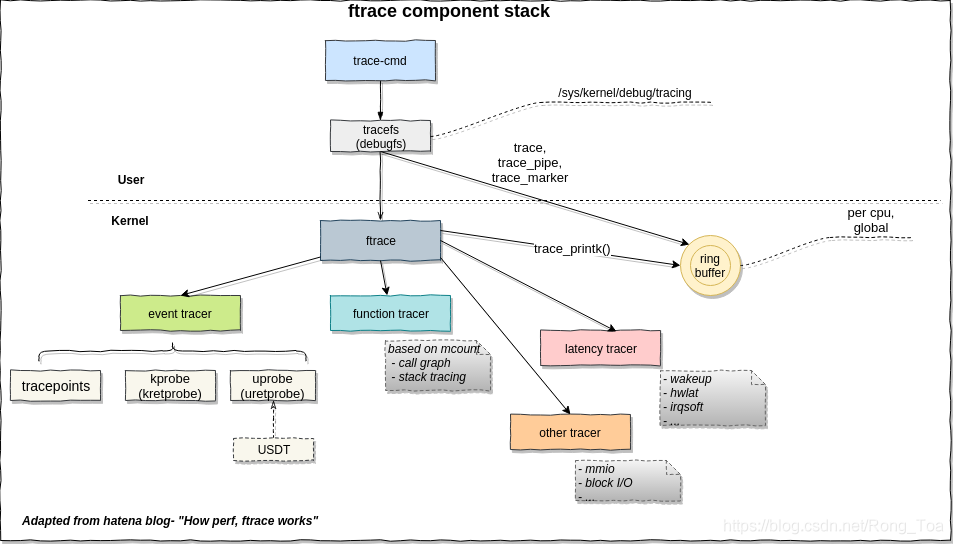
\includegraphics[height=0.3\textheight]{img/ftrace_stack} % height
	\caption{Принцип работы механизма трассировки ftrace}
	\label{img:ftrace_stack}
\end{figure}

Ftrace использует файловую систему tracefs, которая ориентирована на подсистему трассировки и получение доступа к интерфейсу трассировки через каталог без необходимости монтировать debugfs.
При этом создается каталог трассировки <</sys/kernel/debug/tracing>>. Также применяется в ситуациях, когда использования debugfs невозможно из соображения безопасности, т.е. подсистемы ядра могут выводить через debugfs закрытые сведения. 

Для мониторинга сетевой подсистемы ядра Linux с помощью ftrace используется следующий функционал:
\begin{itemize}
	\item function --- трассировщик вызовов функций ядра без возможности получения аргументов;
	\item function\_graph --- трассировщик вызовов функций ядра как function, который показывает все вызовы из определенных фильтров функции, но указывает точку входа и выхода с помощью чего можно отслеживать функции с подвызовами и измерять время выполнения для каждой функции;
	\item blk --- трассировщик вызовов и событий ядра, связанных с вводом-выводом на блочные устройства, а именно использованием утилиты blktrace;
	\item mmiotrace --- трассировщик операций ввода-вывода.
\end{itemize}
Для отслеживания действий сетевой подсистеме лучше использовать трассировщик function\_graph, фильтре которого указывается имя функции, которые участвую в отслеживаемых процессах сетевой подсистемы.   

Использование ftrace не требует модификации кода или добавления дополнительных модулей ядра Linux, поэтому интерфейс является неизменяемым, то есть не зависит от сборки ядра Linux. Самой же противоречивой особенностью ftrace является невозможность добавления пользовательского кода в ядро Linux при трассировке. C одной стороны, благодаря этому повышается безопасность и понижаются расходы ресурсов, но с другой --- ухудшается гибкости под определенную задачу.

\subsubsection{Extended Berkeley Packet Filter}

В 1992 году Стивен Маккейн и Ван Якобсон опубликовали новую архитектуру для захвата пакетов на уровне пользователя, где описали способ реализации фильтра сетевых пакетов для ядра Unix, который работал в 20 раз быстрее, чем все остальные методы фильтрации пакетов.

Berkeley Packet Filter (BPF) --- технология, которая позволяет добавлять программы или модули в ядро Linux без изменения исходного кода ядра~\cite{bpf_for_monitoring}.
BPF представил два серьезных нововведения в области фильтрации пакетов:
\begin{itemize}
	\item новую виртуальную машину (ВМ), предназначенную для эффективной работы с центральным процессором на основе регистров;
	\item возможность использования буферов для каждого приложения способных фильтровать пакеты без копирования всей информации о них.
\end{itemize}

Extended Berkeley Packet Filter (eBPF) расширение реализации BPF, разработанной в 2014 году Алексей Старовойтов. Новый подход был оптимизирован для современного оборудования, благодаря чему результирующий набор команд работает быстрее, чем машинный код, сгенерированный старым интерпретатором BPF. 
Расширенная версия, показанные на рисунке~\ref{img:ebpf}, также увеличила число регистров в виртуальной машине BPF с двух 32-битных регистров до десяти 64-битных. Увеличение количества регистров и их глубины позволило писать более сложные программы, поскольку разработчики могли свободно обмениваться дополнительной информацией, используя параметры функций.
Эти изменения наряду с прочими улучшениями привели к тому, что расширенная версия BPF стала в четыре раза быстрее оригинальной реализации BPF.

\begin{figure}[h!]
	\centering
	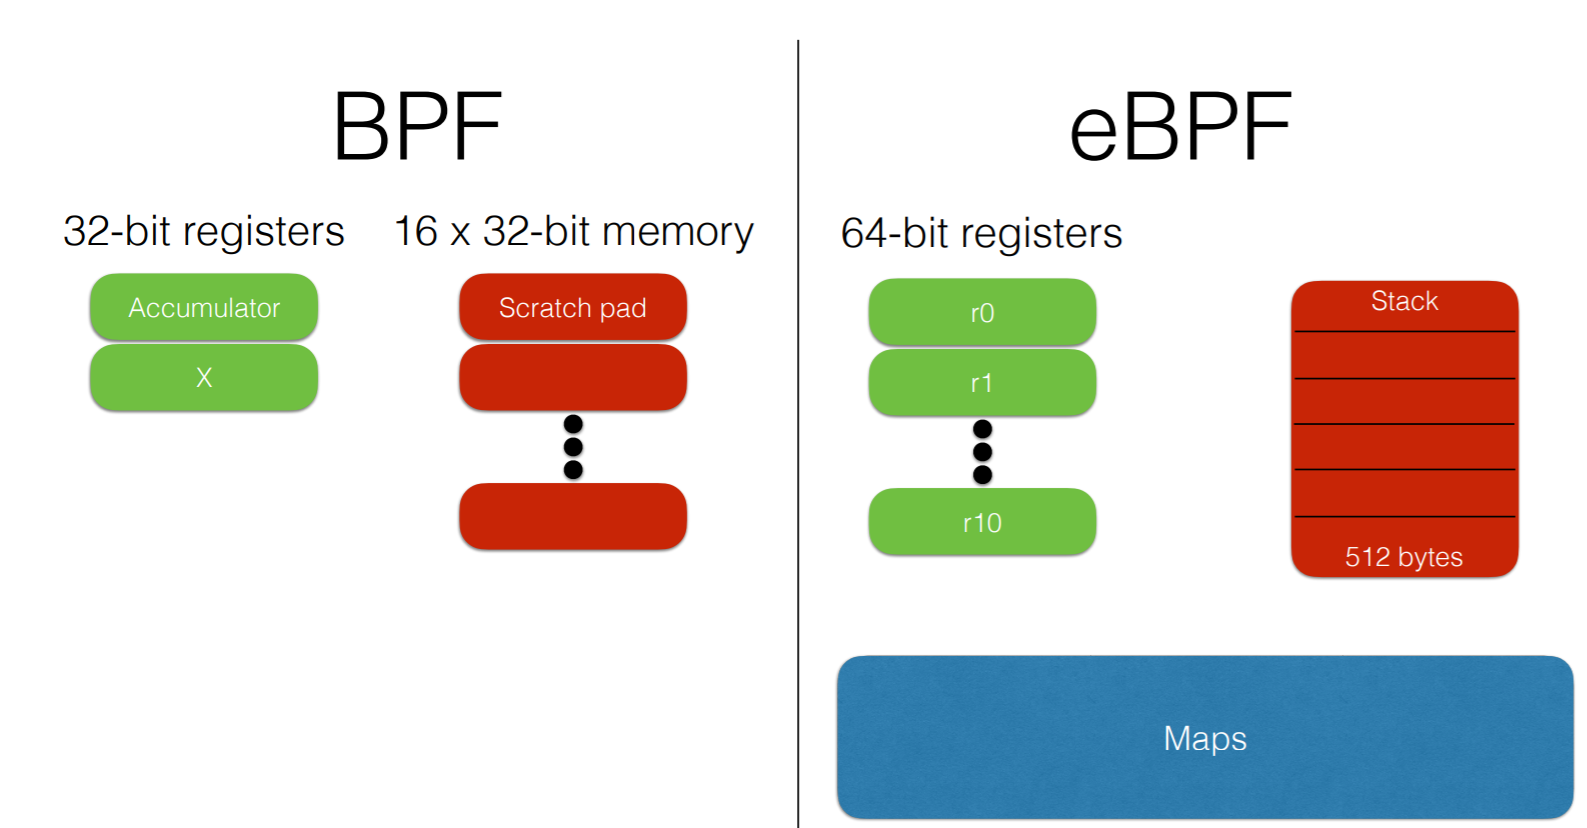
\includegraphics[width=0.8\textwidth]{img/bpf_as_ebpf} % height
	\caption{Отличие между BPF и eBPF технологий}
	\label{img:ebpf}
\end{figure}

eBPF стал подсистемой ядра верхнего уровня в современных ОС Linux и больше походить на модули ядра с сильным акцентом на безопасность, чтобы предотвратить системные сбои и вредоносное поведение каких-либо программ, и стабильность, по причине того что не требует перекомпиляции.

eBPF работает по следующему принципу, показанному на рисунке~\ref{img:arch_bpf}.
В своей основе eBPF использует привилегированную способность ядра видеть и контролировать все ресурсы системы, а компиляторы подобные GNU Compiler Collection (GCC) обеспечивает поддержку BPF, что позволяет скомпилировать код на языке С в байт-код.
С помощью eBPF запускаются изолированные программы в привилегированном контексте, которые используются для доступа к оборудованию и службам из области ядра Linux. 
eBPF позволяет пользовательским приложениям упаковать логику, выполняемую в ядре при возникновении событий.
После компиляции кода приложения использует <<верификатор>>, чтобы убедиться в безопасности для запуска в пространстве ядра. Если код прошел все проверки успешно, программа BPF будет загружена в ядро и преобразована из байт-кода BPF в машинный код с использованием Just-In-Time (JIT) компилятора. 

\begin{figure}[h!]
	\centering
	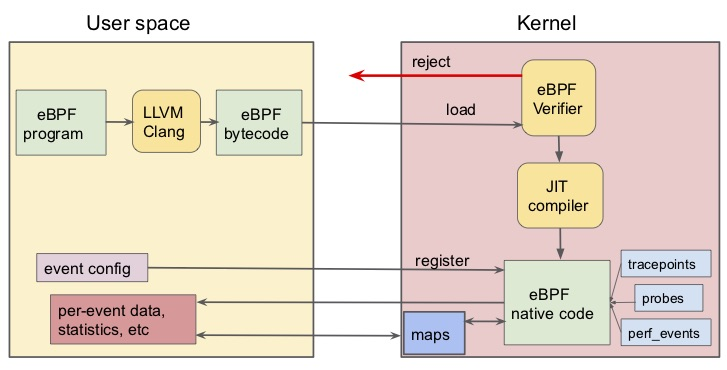
\includegraphics[width=0.9\textwidth]{img/arch_bpf_d}
	\caption{Алгоритм технологии BPF/eBPF}
	\label{img:arch_bpf}
и\end{figure}

Отследить путь сетевого пакета с помощью eBPF использованием два типа: 
\begin{itemize}
	\item программы для работы в сети (Linux Traffic Control);
	\item программы kprobe (зондирования ядра);
	\item программы tracepoint (точки трассировки). 
\end{itemize}

Программы для работы в сети позволяют контролировать сетевой трафик в своей системы, фильтровать и отбрасывать пакеты, поступающие от сетевого интерфейса. Разные программы могут работать по-разному связываться с различными этапами сетевой обработки пакетов в ядре или привязаны к сетевым событиям перед и после передачи или получения пакета. 
Например, программы сокетной фильтрации, привязывают BPF-программы к открытому сокету для получения доступа ко всем пакетам, чтобы наблюдать за информацией сетевого стека. 
Или программы eXpress Data Path (XDP), предоставляющие ограниченный набор информации из пакета, что у ядра было немного времени для ее обработки. Поскольку пакет исследуется и выполняется на ранней стадии, то контроль обработки его намного лучше. 
Реализуют несколько действий по управлению над пакетами и передают подсистеме ядра или игнорируют пакеты.

Программы kprobe, как говорилось ранее, функции, которые можно динамически подключать к определенным точкам вызова в ядре.
Программы типа BPF kprobe позволяют использовать программы BPF в качестве обработчиков kprobe. Виртуальная машина BPF гарантирует, что программы kprobe всегда безопасны при запуске, что является преимуществом по сравнению с традиционными модулями kprobe.

Программы tracepoint, обеспечивающие информацию о поведение системы и оборудования, получаю доступ к области памяти и выполняют трассировку запущенных процессов.
Программы tracepoint позволяют подсоединить BPF-программы к обработчику трассировки, предоставляемым ядром.
Они менее гибки, чем kprobes, потому что должны быть определены ядром заранее, но гарантированно стабильны после введения в ядро соответствующей точки отладки или модуля.
Возможность прикреплять программы eBPF к точкам трассировки в дополнение к точкам тестирования ядра и пользовательских приложений позволяет отслеживать поведение приложений и системы во время выполнения.

Использование eBPF устраняет необходимость модификации исходного кода ядра и повышает возможности программного обеспечения по обеспечению безопасности при исполнении, то есть любая BPF-программа завершится без сбоев и программы не будут пытаться получить
доступ к памяти вне области их деятельности, и реализации запуска на работающей систему.
Но эти преимущества сопровождаются определенными ограничениями: программы имеют максимально допустимый размер, и циклы должны быть ограничены, чтобы гарантировать, что память системы никогда не будет исчерпана неправильно написанной программой BPF.
Кроме того, при использовании eBPF наблюдается небольшое снижение производительности, поскольку программы пишутся в байт-коде BPF, а затем интерпретируются в ядре. Однако этот разрыв стал еще меньше теперь, когда eBPF поддерживает компиляцию JIT, что позволяет избавиться от фильтрации пакетов в каждой функции тем самым достичь низких накладных ресурсов.
Данная технология позволяет разными программами выполнить требования к обработке сетевых пакетов.
Изменение программ для фильтрации пакетов осуществляет работу при нужной нагрузке.
eBPF не зависит от реализации ядра, что способствует независимости от конкретной сборки.
Однако eBPF – молодой и пока еще развивающийся инструмент. В связи с этим в ходе разработки eBPF-программ могут возникать проблемы, связанные с отсутствием нужного инструментария, документации или её недостаточной информативностью.

\subsection{Критерии сравнения методов сетевого мониторинга}

В данном разделе будут описаны критерии, которые будут использоваться для сравнения подсистем и средств сетевого мониторинга ядра.

\begin{table}[ht]
	\begin{center}
		\begin{threeparttable}
			\caption{\label{tb:criteria}Критерии сравнения методов сетевого мониторинга}
			\begin{tabular}{|c|p{8cm}|}
				\hline
				\textbf{Критерий} & \textbf{Описание} \\ \hline
				\textbf{Производительность} & Работа при реальной нагрузки и низкие расход системных ресурсов. \\ \hline
				\textbf{Безопасность} & Наличие гарантии, что внесенный код не вызовет сбой системы или нет необходимости к внедрению написанного кода \\ \hline
				\textbf{Скорость разработки} & Быстрота разработки программ для сетевого мониторинга \\ \hline
				\textbf{Работоспособность} & Запуск на работающей системе без сбоев или требования перезапуска \\ \hline
				\textbf{Гибкость} & Возможность выполнить любые поставленные задачи \\ \hline
				\textbf{Независимость} & Независимость от сборки ядра \\ \hline
				\textbf{Простота развертывания} & Насколько сложно развертывать средства мониторинга на машине и сопровождением документации \\ \hline
			\end{tabular}
		\end{threeparttable}
	\end{center}
\end{table}

\clearpage

\subsection{Сравнение методов сетевого мониторинга}

\begin{table}[ht]
	\begin{center}
		\begin{threeparttable}
			\caption{\label{tab:comparison_1} Сравнение методов сетевого мониторинга (Часть 1)}
			\begin{tabular}{|c|c|c|c|}
				\hline
				\textbf{Критерий}            	& \textbf{Утилиты} 			 & \textbf{ftrace}    & \textbf{BPF / eBPF} \\ \hline
				\textit{Производительность}  	& \cmark\footnotemark		 & \cmark 			& \cmark 			\\ \hline
				\textit{Безопасность}        	& \cmark 		   			 & \cmark 			& \cmark 			\\ \hline
				\textit{Скорость разработки} 	& ---\footnotemark 			 & --- 				    & \cmark 			\\ \hline
				\textit{Работоспособность}   	& \cmark 		   			 & \cmark 			& \cmark 			\\ \hline
				\textit{Гибкость}            	& \xmark\footnotemark 	     & \xmark 			& \xmark 			\\ \hline
				\textit{Независимость}   	 	& \cmark/\xmark\footnotemark & \cmark 			& \cmark 			\\ \hline
				\textit{Простота развертывания} & \cmark 		   			 & \xmark 			& \cmark 			\\ \hline
			\end{tabular}
		\end{threeparttable}
	\end{center}
\end{table}


\begin{table}[ht]
	\begin{center}
		\begin{threeparttable}
			\caption{\label{tab:comparison_2} Сравнение методов сетевого мониторинга (Часть 2)}
			\begin{tabular}{|c|c|c|c|}
				\hline
				\textbf{Критерий}            	& \textbf{Модификация} & \textbf{kprobes} & \textbf{tracepoint} \\ \hline
				\textit{Производительность}  	& \cmark/\xmark 	   & \cmark/\xmark 	  & \cmark 			    \\ \hline
				\textit{Безопасность}        	& \xmark 		       & \cmark/\xmark 	  & \cmark/\xmark 		\\ \hline
				\textit{Скорость разработки} 	& \xmark 		       & \xmark  	      & \cmark 			    \\ \hline
				\textit{Работоспособность}   	& \cmark/\xmark	       & \cmark/\xmark 	  & \cmark/\xmark 		\\ \hline
				\textit{Гибкость}            	& \xmark 		       & \cmark 		  & \cmark 			    \\ \hline
				\textit{Независимость}   	 	& \xmark               & \cmark/\xmark 	  & \cmark 				\\ \hline
				\textit{Простота развертывания} & \cmark 		       & \cmark/\xmark 	  & \cmark/\xmark 		\\ \hline
			\end{tabular}
		\end{threeparttable}
	\end{center}
\end{table}

\footnotetext[1]{Метод сетевого мониторинга ядра Linux в реализации данного критерия полностью возможно.}
\footnotetext[2]{Метод сетевого мониторинга не требует изменение или добавление пользовательского кода в ядро Linux.}
\footnotetext[3]{Метод сетевого мониторинга ядра Linux в реализации данного критерия полностью невозможна либо значительно осложнена в сравнении с остальными методами.}
\footnotetext[4]{Метод сетевого мониторинга ядра Linux в реализации данного критерия возможно, но осложнена.}
